\graphicspath{ {./figuresConception} }
\section{Conception}

\subsection{Circuit}
L'objectif de ce travail est d'analyser et de valider le principe physique de notre capteur. Nous nous contrerons principalement sur le dipôle. Nous établissons un schéma électrique du capteur pour nous aider lors du câblage des cartes de développement. Ce schéma ne comporte pas la gestion de l'alimentation car ce qui nous intéresse est la chaîne de mesure.

\begin{figure}[!ht]
 \centering
 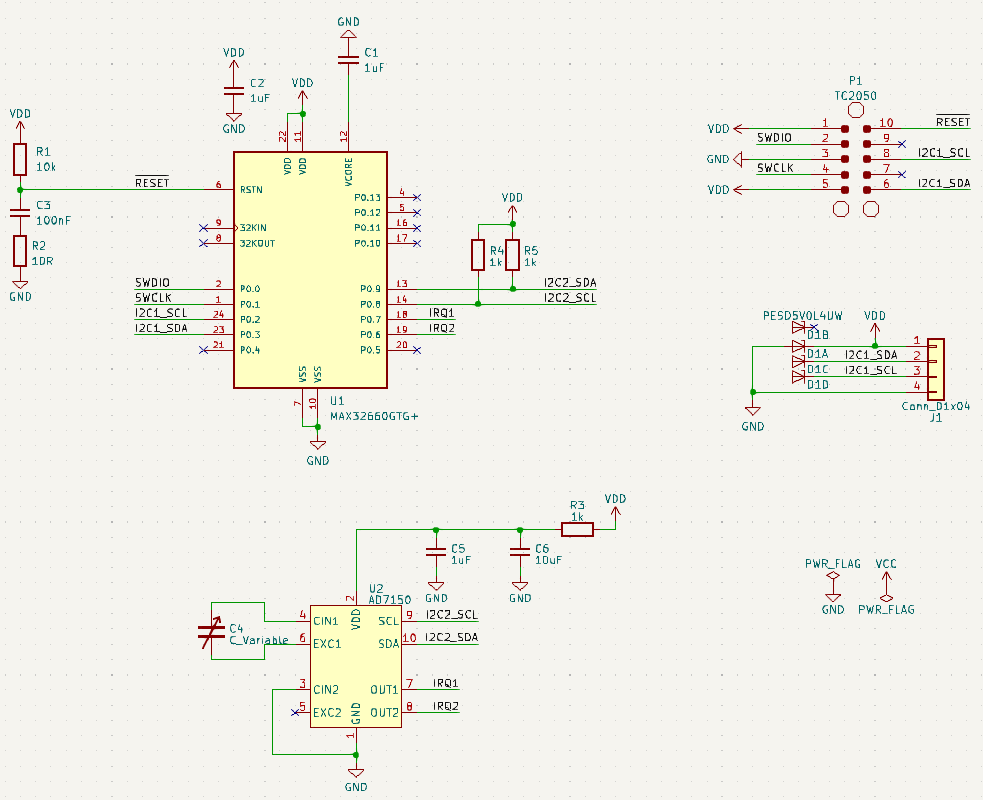
\includegraphics[width=14cm]{schemaelec.png}
 \caption{Schéma électrique}
\end{figure}

Sur ce schéma C4 représente le dipôle. Il est connecter sur le premier port du convertisseur. Un pôle est connecter sur la pin d'excitation et l'autre sur l'entrée analogique. La conversion est faites en excitant d'un côté et en mesurant la charge de l'autre. La valeur est stocké dans un registre prête à être lu par l'I2C. Un filtre conseillé par la datasheet est câblé sur l'alimentation de l'AD7150. Le micro-contrôleur est connecter aux convertisseur par les deux pin de l'I2C, clock et donnée. On utilise le deuxième I2C pour le convertisseur et le premier pour l'interface extérieur. Les pull-up obligatoire sont connecter sur le deuxième I2C mais pas sur le premier car elle se trouve déjà aux niveau de l'émetteur. Les deux sortie numérique sont aussi connecter au micro-contrôleur. Nous ne les utiliserons pas tout de suite mais nous nous en laissons la possibilité. Le connecteur P1 est un tag pour flasher le micro. Il est relié aux pin nécessaire pour sa tâche et à l'I2C d'interface à des fin de debug. Et finalement le connecteur J1 permet de sortir l'interface I2C et apporte l'alimentation. Des diode protège le circuit contre les surtensions.  

\newpage
\subsection{Dipôle}
Le dipôle est la partie de notre capteur qui transforme une variable physique en un paramètre électrique. Dans notre cas il transforme une quantité d'eau sur la surface en une variation de capacité. Pour comprendre comment cela fonctionne il faut comprendre ce qu'est une capacité électrique. $C=\frac{Q}{U}$ défini la capacité (C) comme la charge (Q) stocké par rapport à une tension (U) donné. La capacité d'un dipôle est influencé par trois paramètres. La surface du conducteur l'augmente. La distance entre deux pôle la diminue. Et enfin, Une plus grande permittivité relative du milieux augmentera le milieux. L'eau fera varier ce dernier paramètres ce qui nous laisse les deux autres à définir.

Le dipôle sera d'abord simulé puis mesuré. La simulation se fera avec le logiciel Flux d'Altair. Pour simplifié la simulation nous l’exécuterons en 2 dimension. Ce premier dipôle devra être conçu pour qu'une coupe 2d puisse être utilisé dans la simulation. Nous choisiront un peigne droit en longueur. 

\begin{figure}[!ht]
 \centering
 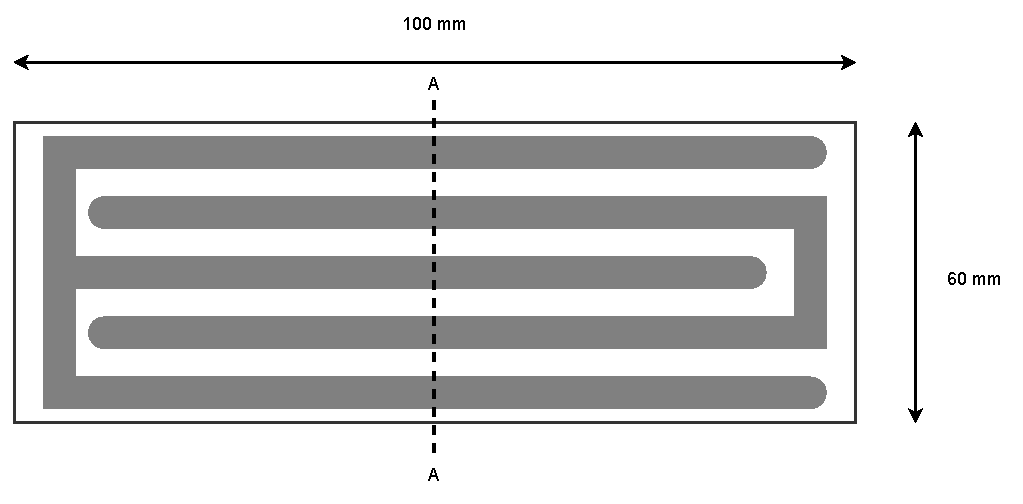
\includegraphics[width=14cm]{dipole-top.pdf}
 \caption{Plan mécanique du dipôle}
 \label{plan}
\end{figure}

Nous avons défini arbitrairement une longueur de 100mm et une largeur de 60mm. Cette taille nous donne un bon compromis entre l'espace disponible sur la carte et le prix de production. 

\begin{figure}[!ht]
 \centering
 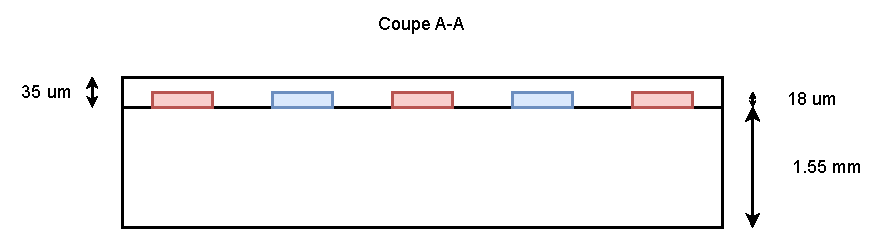
\includegraphics[width=14cm]{dipole-A-A.pdf}
 \caption{Plan mécanique de coupe du dipôle}
 \label{plancoupe}
\end{figure}

Les différentes épaisseurs des couches, du PCB, du cuivre et du masque sont récupéré à partir des dimension de carte standard. C'est cette coupe que nous simulerons dans le logiciel. Cependant nous ajouterons une couche de résine supplémentaire de 0.5 mm d'épaisseur. Elle permettra sur le capteur final de protéger le circuit et d'offrir à l'eau une surface proche de celle de l'eau en terme d'étanchéité et de rugosité. Cette couche ne sera pas présente pour nos première mesures. Mais doit être pris en compte pendant la simulation. Nous évaluerons aussi l'utilisation d'un plan conducteur pour concentré le champs en direction de la surface mesuré et éviter que le capteur sois influencé par ce qui se passe en dessous. Nous prendrons la décision de garder ou non cette couche après l'avoir simulé et étudié.

Le nombre, l'épaisseur, et l'écart des pistes sont des valeurs que nous laissons libre pour la simulation. La coupe ne représente que la partie centrale du PCB. Pour un question de simplicité nous négligerons les extrémité pour les simulations.

